\section{Introduction}

From 2009 to 2013 the Kelper Space Telescope looked almost continualy at one point in space. Its goal was to measure the magnitude of a large number of stars with a high frequency for 4 years in order to examine the exoplanets (planets orbiting stars other than the sun) similar to Earth. \\
\\
This report examines the time series of data taken by the Kepler Space Telescope in order to exaimne the effects of Finite Impulse Responce (FIR) and Infinite Imuplse Responce (IIR) filters. The data is choosen to be a different type of signal from what we usually see, and it is therefore not expected that any results of scientific relevance is acheived.\\
\\
In the following we will examine the design of a FIR filter, and how FIR and IIR filters affects the time series. 


\section{Time series and spectrum}

The data series we examine is shown in \autoref{fig:time_series}. The time axis is in bariocentric julian days (BJD) with an offset of 2454833 days (bringing 0 to 1/1/2009). The y-axis is photometric flux, meassured in $\frac{e^-}{s}$. It can be seen that the data undergoes a general drift, increasing in magnitude as time passes.

\begin{figure}[h]
    \centering
    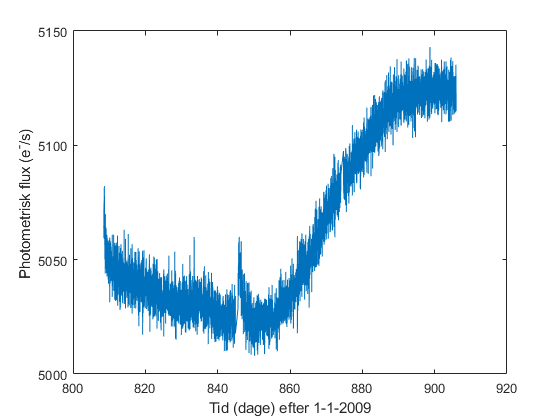
\includegraphics[width = \textwidth]{kep_timeseries.png}
    \caption{Kepler time series}
    \label{fig:time_series}
\end{figure}

The discrete fourier transform (DFT) of the timeseries is displayed in \autoref{fig:smooth_spec}. Note that the frequency is in $\frac{1}{day}$ rather than the usual Hz. This is due to the timeseries being sampled in fractions of days (arround once every half hour (or 0.00056 Hz)).\\
It can be seen in the figure that there is a rather large component with a low frequency. This is probably caused by the general drift in the data.\\ 

\begin{figure}[h]
    \centering
    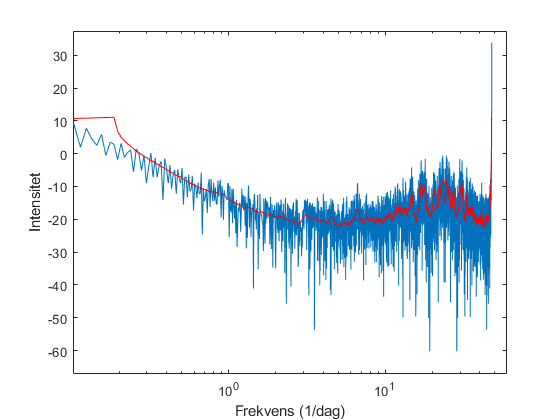
\includegraphics[width = \textwidth]{smooth_spectrum.png}
    \caption{Spectrum of the simeseries and the same spectrum smoothed vit a binsize of 35}
    \label{fig:smooth_spec}
\end{figure}

\autoref{fig:smooth_spec} also shows a smoothed spectrum, with a binsize of 35. It is clear that there is some irregularity in the low frequencies, probably a result of the smoothing including parts beyond the spectrum.\\

The smoothed spectrum removes a large amount of (presumably) noise from the spectrum and highligts a number of peaks. As the timeseries is from a planet survey, it is probable that one or more of these peaks are caused by an eclipse.

\newpage
